% Options for packages loaded elsewhere
\PassOptionsToPackage{unicode}{hyperref}
\PassOptionsToPackage{hyphens}{url}
%
\documentclass[
]{article}
\usepackage[a4paper, margin=2cm]{geometry}
\usepackage{amsmath,amssymb}
\usepackage{lmodern}
\usepackage{tabularray}
\usepackage{tabularx}
\usepackage{iftex}
\ifPDFTeX
  \usepackage[T1]{fontenc}
  \usepackage[utf8]{inputenc}
  \usepackage{textcomp} % provide euro and other symbols
\else % if luatex or xetex
  \usepackage{unicode-math}
  \defaultfontfeatures{Scale=MatchLowercase}
  \defaultfontfeatures[\rmfamily]{Ligatures=TeX,Scale=1}
\fi
% Use upquote if available, for straight quotes in verbatim environments
\IfFileExists{upquote.sty}{\usepackage{upquote}}{}
\IfFileExists{microtype.sty}{% use microtype if available
  \usepackage[]{microtype}
  \UseMicrotypeSet[protrusion]{basicmath} % disable protrusion for tt fonts
}{}
\makeatletter
\@ifundefined{KOMAClassName}{% if non-KOMA class
  \IfFileExists{parskip.sty}{%
    \usepackage{parskip}
  }{% else
    \setlength{\parindent}{0pt}
    \setlength{\parskip}{6pt plus 2pt minus 1pt}}
}{% if KOMA class
  \KOMAoptions{parskip=half}}
\makeatother
\usepackage{xcolor}
\IfFileExists{xurl.sty}{\usepackage{xurl}}{} % add URL line breaks if available
\IfFileExists{bookmark.sty}{\usepackage{bookmark}}{\usepackage{hyperref}}
\urlstyle{same} % disable monospaced font for URLs
\usepackage{longtable,booktabs,array}
\usepackage{calc} % for calculating minipage widths
% Correct order of tables after \paragraph or \subparagraph
\usepackage{etoolbox}
\makeatletter
\patchcmd\longtable{\par}{\if@noskipsec\mbox{}\fi\par}{}{}
\makeatother
% Allow footnotes in longtable head/foot
\IfFileExists{footnotehyper.sty}{\usepackage{footnotehyper}}{\usepackage{footnote}}
\makesavenoteenv{longtable}
\usepackage{graphicx}
\makeatletter
\def\maxwidth{\ifdim\Gin@nat@width>\linewidth\linewidth\else\Gin@nat@width\fi}
\def\maxheight{\ifdim\Gin@nat@height>\textheight\textheight\else\Gin@nat@height\fi}
\makeatother
% Scale images if necessary, so that they will not overflow the page
% margins by default, and it is still possible to overwrite the defaults
% using explicit options in \includegraphics[width, height, ...]{}
\setkeys{Gin}{width=\maxwidth,height=\maxheight,keepaspectratio}

% Set default figure placement to htbp
\makeatletter
\def\fps@figure{htbp}
\makeatother
\setlength{\emergencystretch}{3em} % prevent overfull lines
\providecommand{\tightlist}{%
  \setlength{\itemsep}{0pt}\setlength{\parskip}{0pt}}
  
% \setcounter{secnumdepth}{-\maxdimen} % remove section numbering

\ifLuaTeX
  \usepackage{selnolig}  % disable illegal ligatures
  \usepackage{rotating}
  \usepackage{amsmath,amssymb} % For mathematical symbols and equations
\usepackage{graphicx} % For including images
\usepackage{float} % To control figure placement
\usepackage{longtable,booktabs,array} % For advanced table formatting
\usepackage{xurl} % Add URL line breaks if available
\usepackage{hyperref} % For hyperlinks
\fi


\title{\LARGE \textbf{Escape Doom - Software Architecture}}
\author{Kambal, Nowak, Perov, Selbach, Winter}
\date{\today}

\begin{document}
\maketitle

% --- Table of contents autogenerated ------------------------------------
\newpage
\tableofcontents

\hypertarget{section-introduction-and-goals}{%
\section{Project-Vision and Goals}\label{section:introduction-and-goals}}

The Escape Doom system aims to provide FH Campus Wien with a platform for creating educational escape rooms. In the first semester of our Bachelor’s program, we participated in a programming escape room that offered an engaging, interactive learning experience. Inspired by this positive experience, we want to create a platform that allows students to easily access and play similar escape rooms.


\subsection{Motivation}

Initially, instructors of FH Campus Wien manually created and managed escape rooms by coding each one from scratch. This approach allows for unique, tailored experiences, but it is labor-intensive and difficult to maintain over time, especially as riddles need to be refreshed every one to two years to prevent sharing of solutions between cohorts. This inspired us to develop our own version of an escape room to explore the potential for creating a scalable, reusable platform.

In the current situation, our project—while functional—still requires participants to use an IDE (with the code accessible) which limits usability and makes solutions to code-based challenges more easily discoverable. Our goal is to address these limitations by transforming the project into a streamlined, maintainable system—or in other words, a product—that reinforces the educational value of the escape room.

\subsection{Product Vision}

Our target groups include both students and instructors at FH Campus Wien. For students, we aim to create an escape room platform that enhances learning by providing a fun, interactive environment with near real-time collaboration and an intuitive, browser-based coding experience. For instructors, we aim to provide a maintainable system that allows them to use escape rooms as an educational tool, with the future goal of enabling them to design and configure their own escape rooms.

Our vision is to develop a tool that enables instructors to create and manage user-friendly and accessible point-and-click escape rooms for their courses, with functionality similar to CodinGame escape rooms.\footnote{\url{https://escape.codingame.com/}}



\begin{figure}[h!]
    \centering
    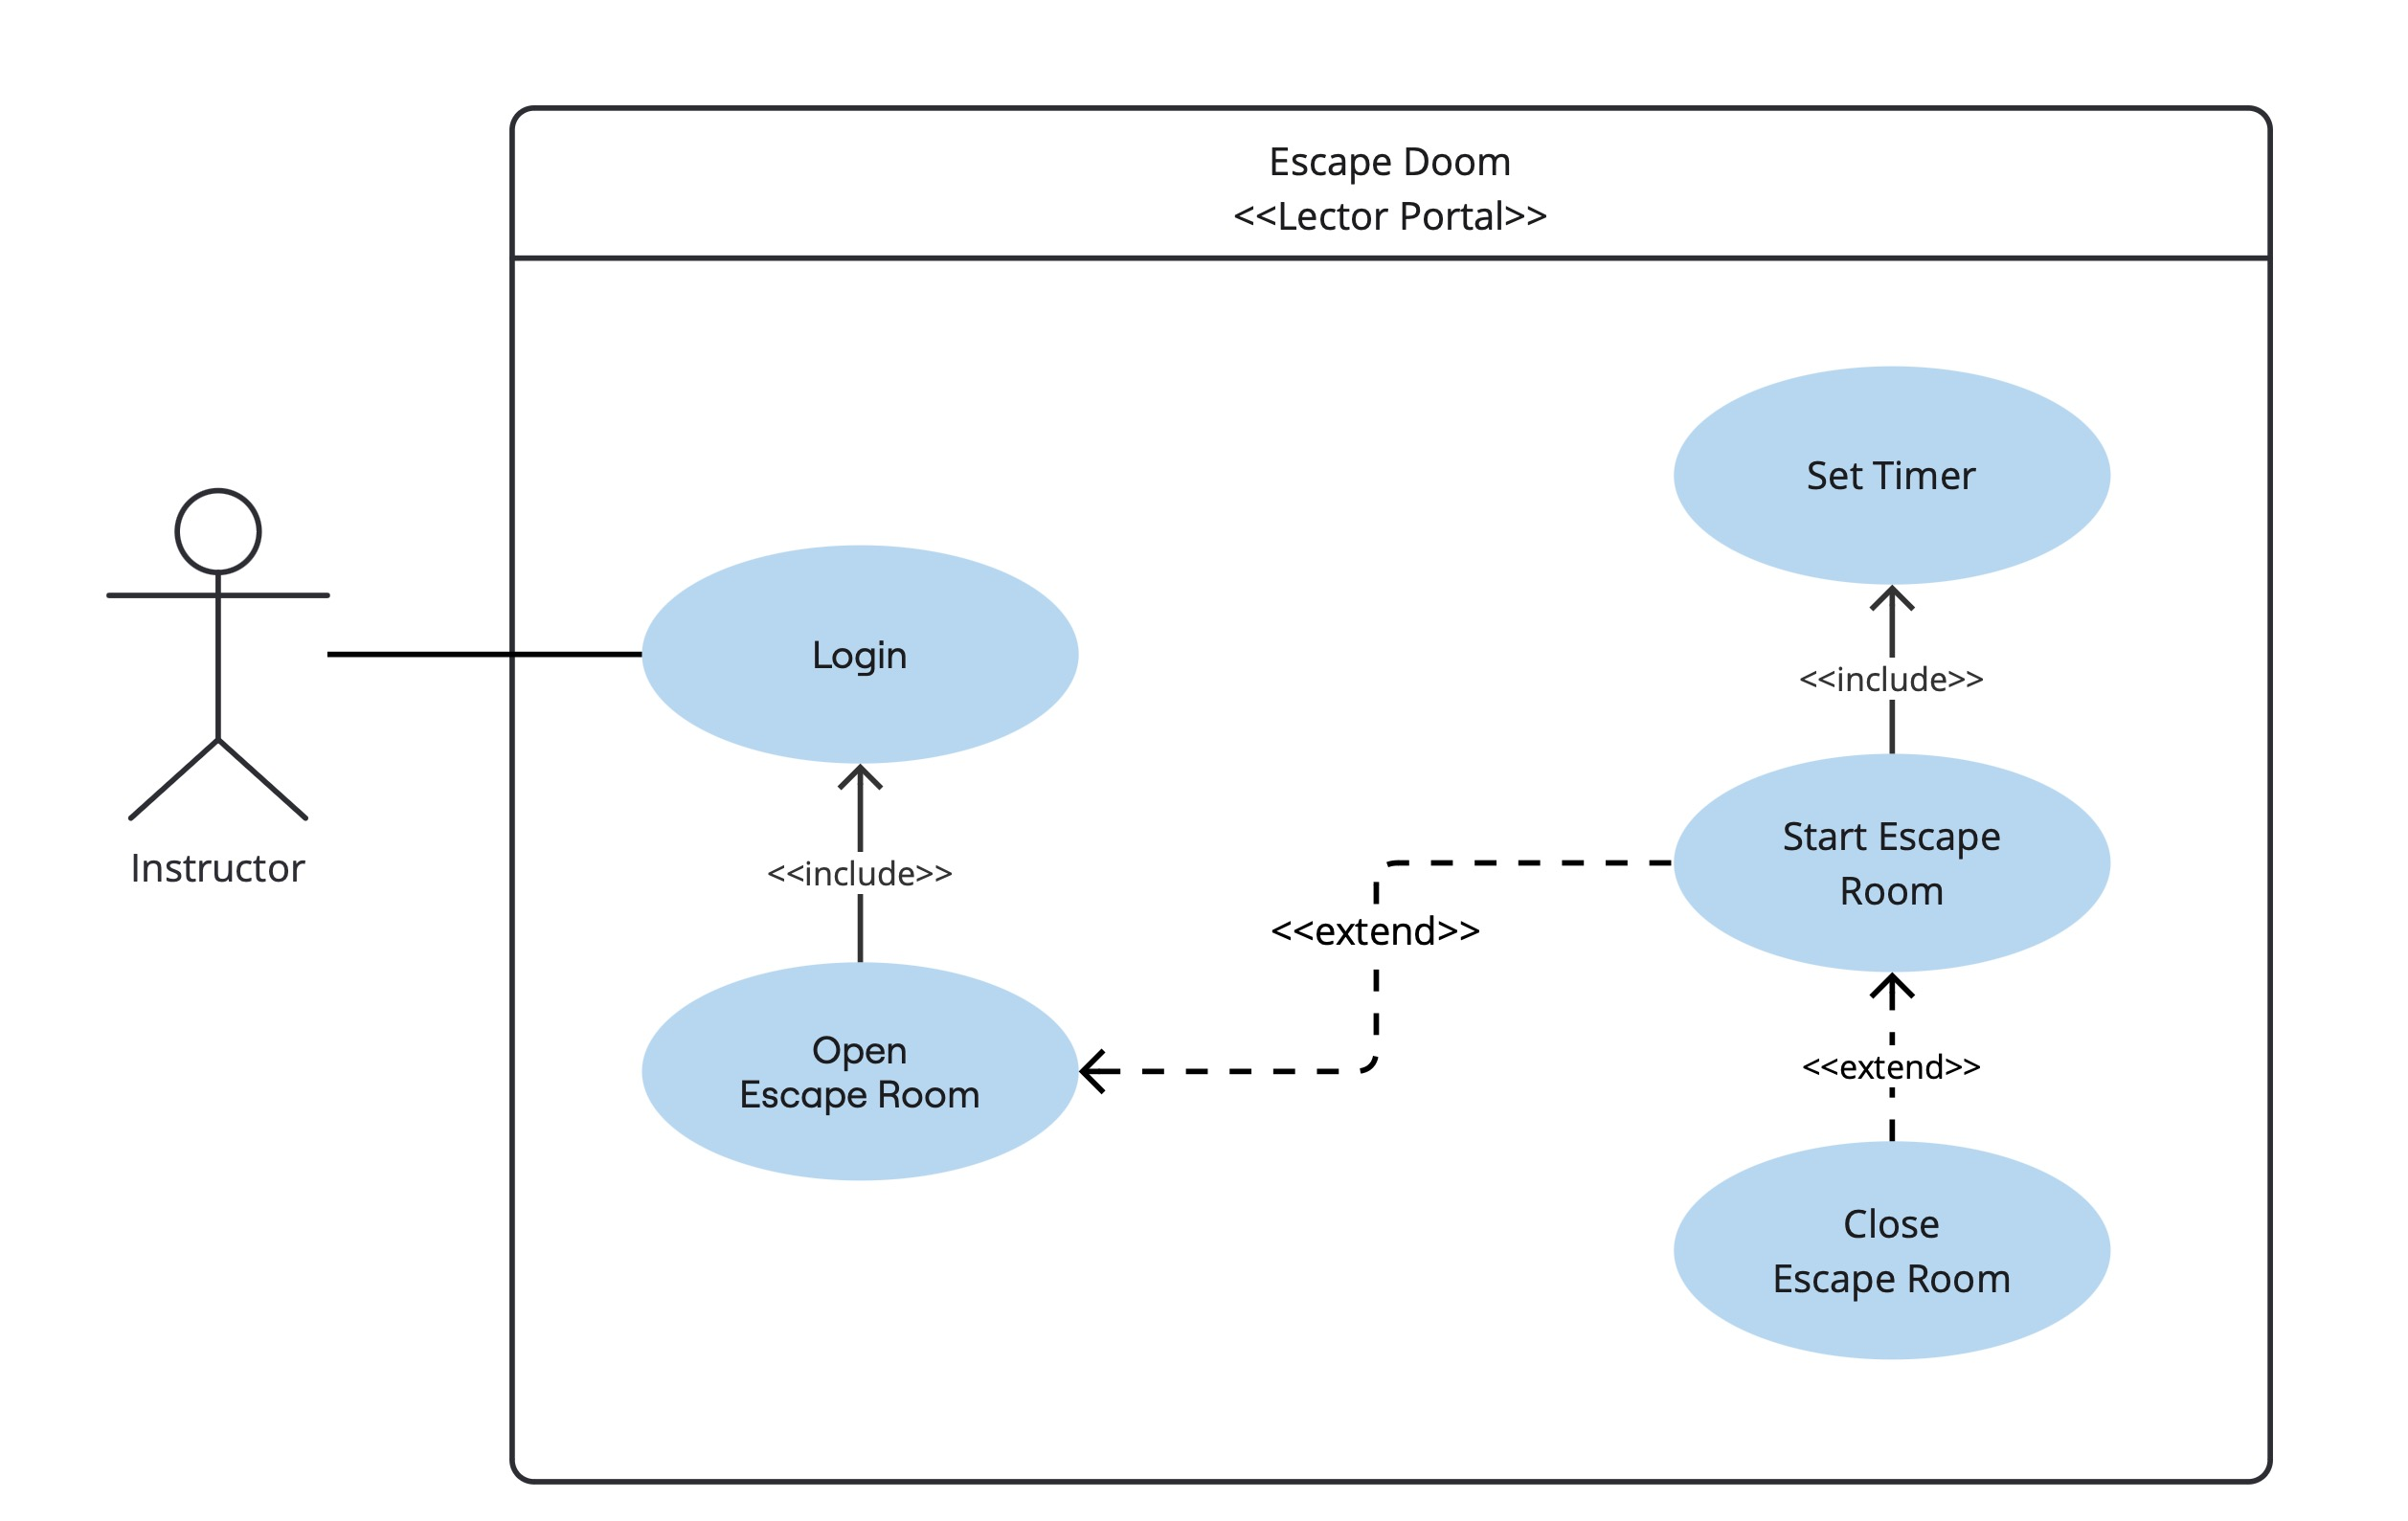
\includegraphics[width=\linewidth]{UC-01.png}
    \caption{UC01 - Lector Portal}
    \label{fig:uc-01}
\end{figure}



\begin{figure}[h!]
    \centering
    \includegraphics[width=\linewidth]{images/LectorPortal.png}
    \caption{Lector Portal Mockup}
    \label{fig:lector:portal}
\end{figure}


\begin{figure}[h!]
    \centering
    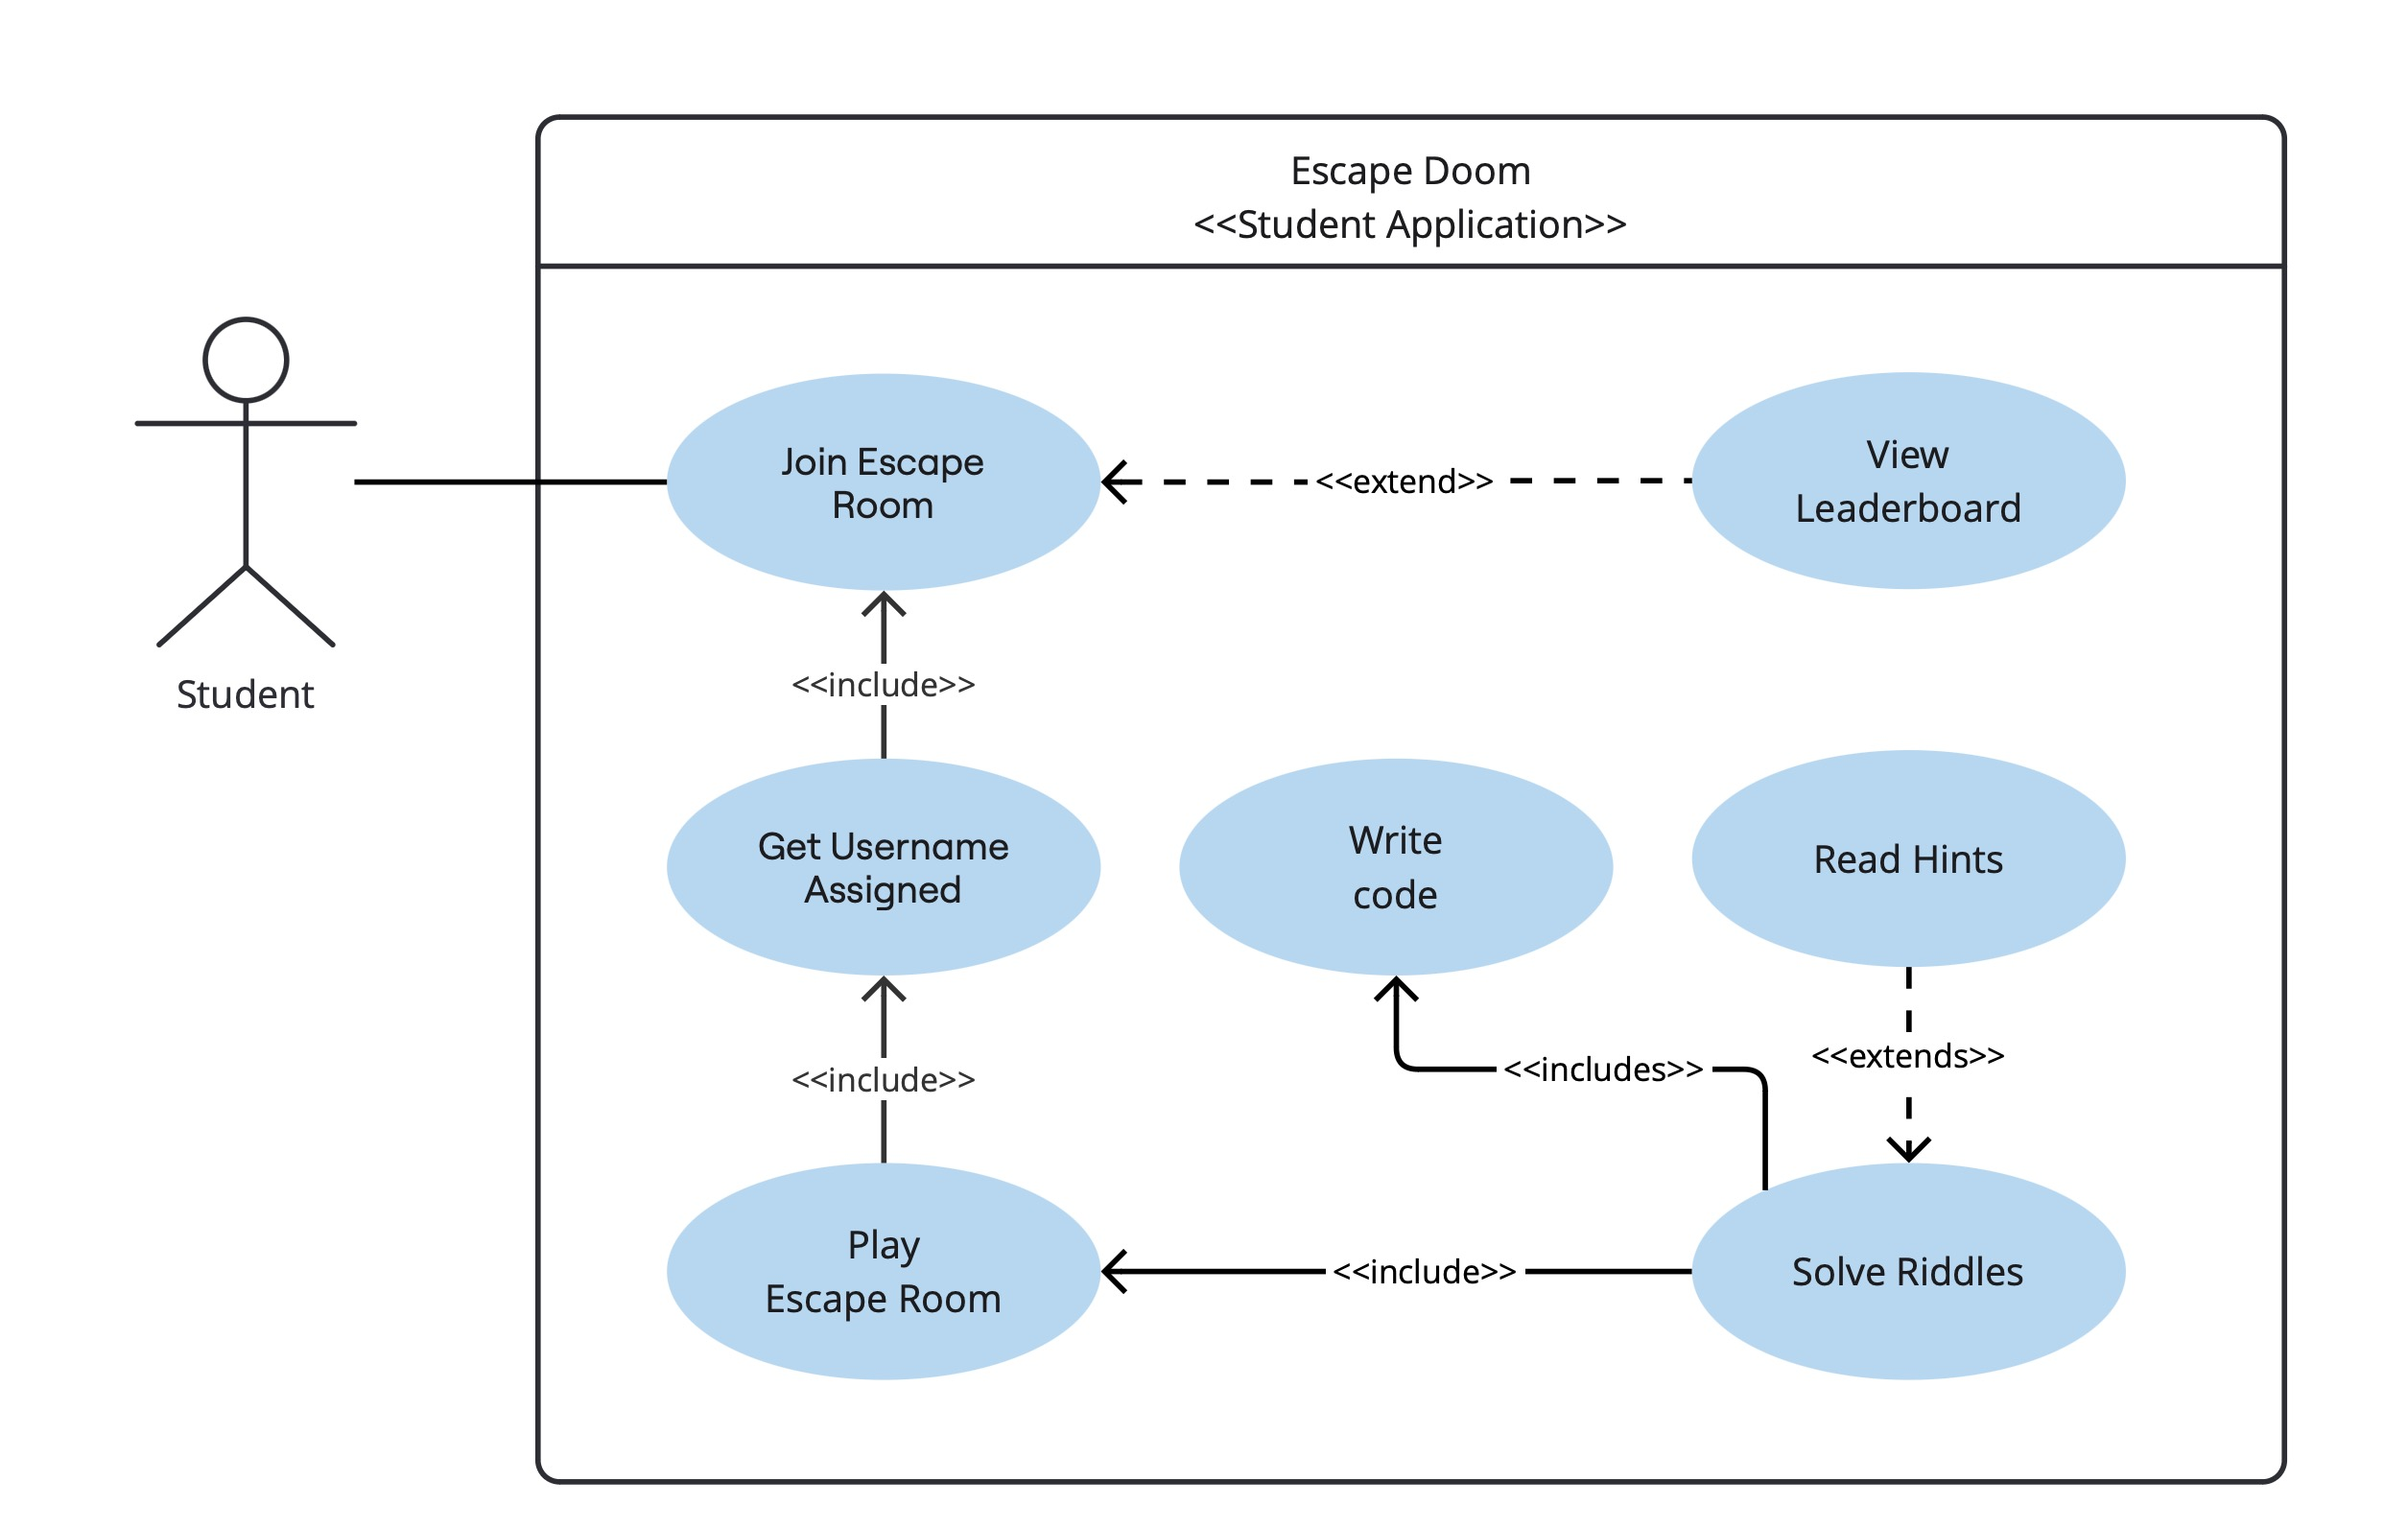
\includegraphics[width=\linewidth]{UC-02.png}
    \caption{UC02 - Student Application}
    \label{fig:uc-02}
\end{figure}
\newpage

\begin{figure}[h!]
    \centering
    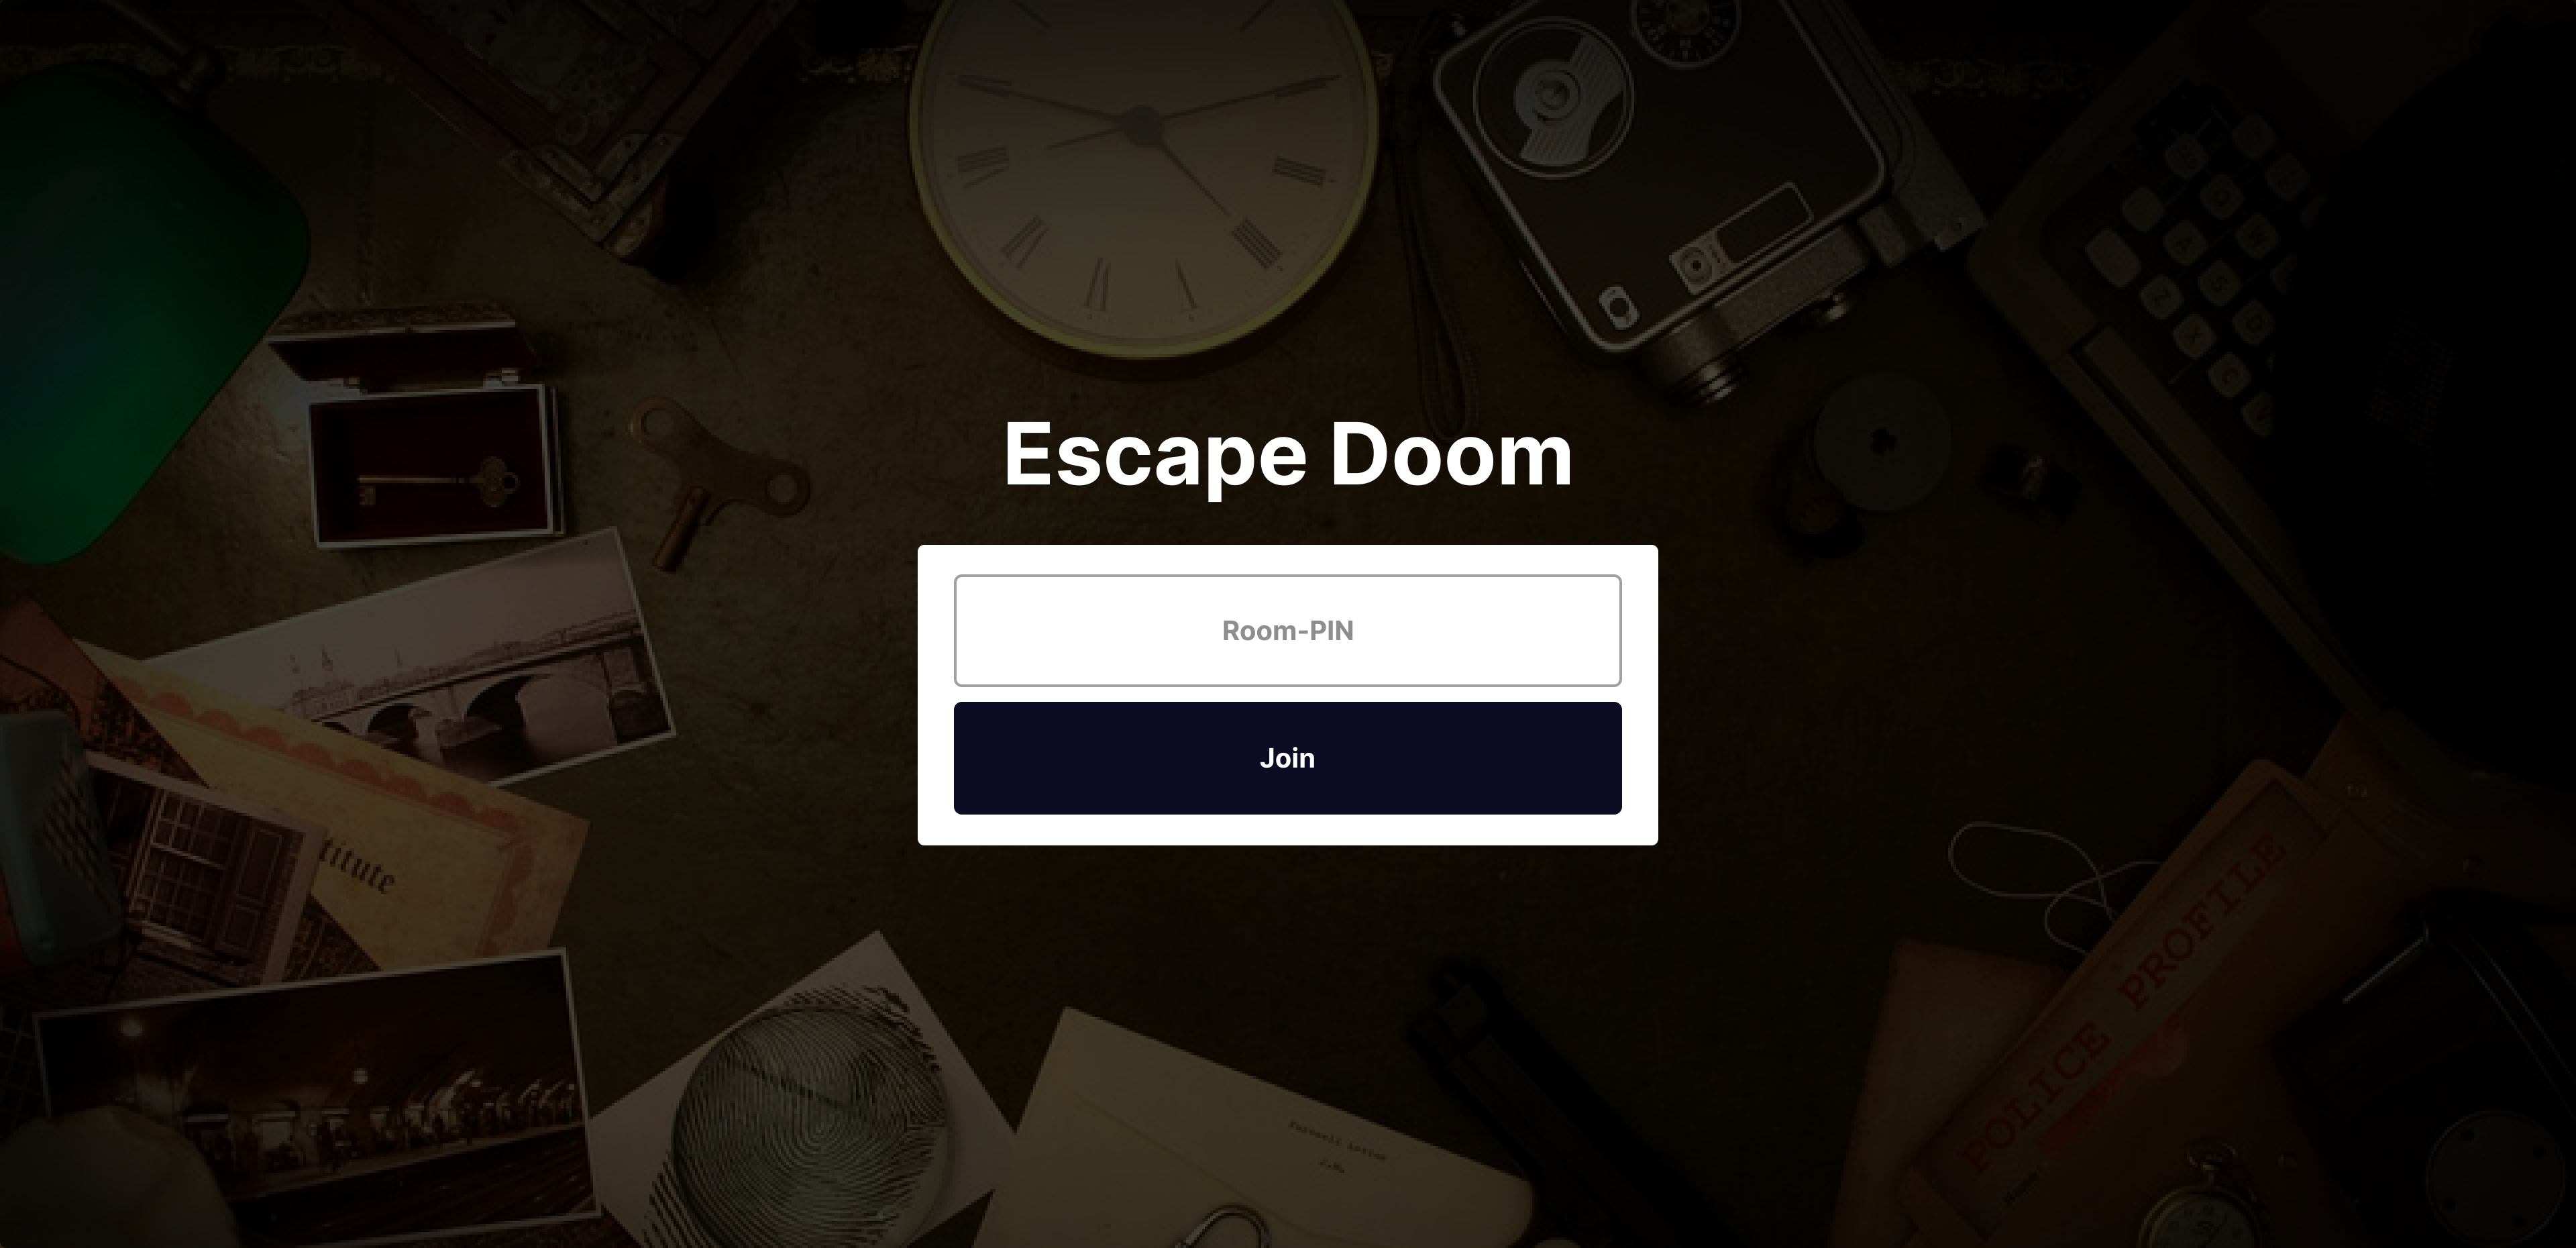
\includegraphics[width=\linewidth]{images/StudentJoin.png}
    \caption{Student Application Mockup}
    \label{fig:lector:portal}
\end{figure}

\hypertarget{section-context-and-scope}{%
\section{Context and Scope}\label{section-context-and-scope}}

\hypertarget{_business_context}{%
\subsection{Business context}\label{_business_context}}
\begin{figure}
    \centering
    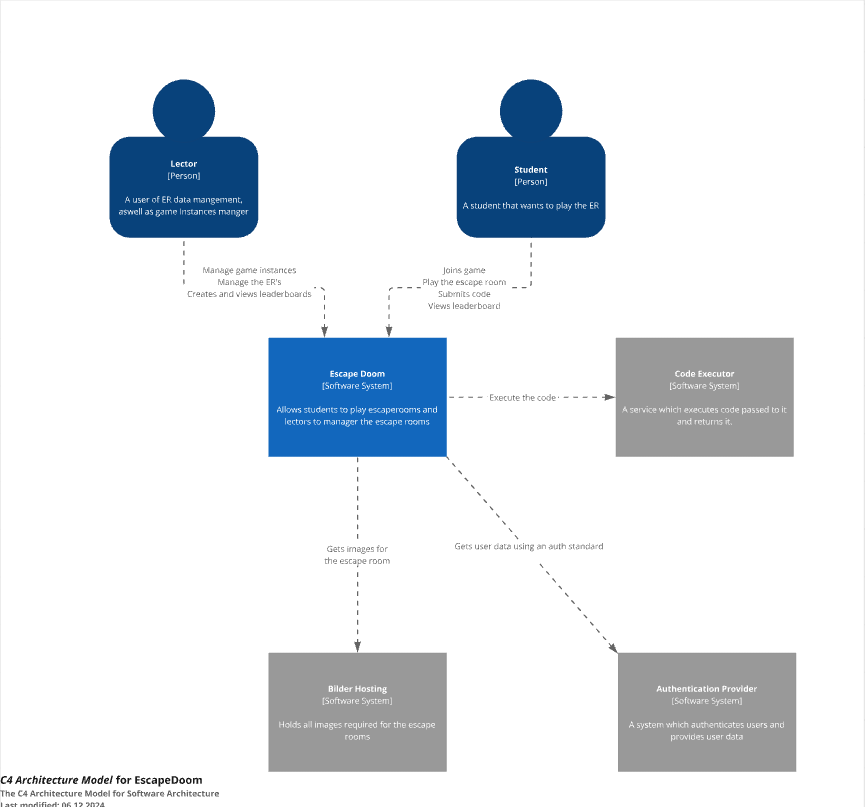
\includegraphics[width=1\linewidth]{C4-Layer1.png}
    \caption{Context diagram with C4 Notation}
    \label{fig:enter-label}
\end{figure}

\newpage

\hypertarget{section-solution-strategy}{%
\section{Solution Strategy}\label{section-solution-strategy}}

To fulfill the task of providing a microservices system which is also maintainable, the team constructed some guiding principles.

\begin{enumerate}
    \item All backend services from the escape room domain will be written in Spring Boot. To achieve the quality goal of easy maintainability. Because only framework needs to be understood when developing in the system.
    \item Since the focus of our project is to build a microservice system the frontend is a single Next.js application, which serves as our only client for students as well as lectors.
    \item The system is split into microservices by grouping the business needs in scalable units of compute. This was the choice to enjoy the rapid elasticity and scalability of the architecture pattern.
    \item The system itself is being split by business needs, and therefore runtime dependency is a side effect the team is accepting for faster iterations and architecture overhead.
    \item The cloud technology used to enable microservices development with the largest velocity possible is the spring cloud ecosystem with a strong emphasis on the Spring cloud Gateway. For efficent  and easy custmizable service routing.
    \item The deployment is on a Kubernetes cluster and, therefore all systems are built stateless and the state is externalized in systems like redis and Postgres-sql.
    \item The Code Executor is a system developed by us but seen as an external system since it is an already solved sub-domain and also could easily be swapped with a finished project. Instead of the own implementation. To support this flexibility, we have also implemented an interface that allows integration with external APIs capable of compiling and executing code.
\end{enumerate}

\hypertarget{section-building-block-view}{%
\section{Building Block View}\label{section-building-block-view}}

\subsection{Level 1 - Context}\label{sub:5:l1}

EscapeDoom is developed with the intent to not create/maintain all parts it requires. Systems such as image hosting or the authentication provider are not part of the EscapeDoom software system, as can be seen in figure \ref{fig:c4:c1} below.

\begin{figure}
    \centering
    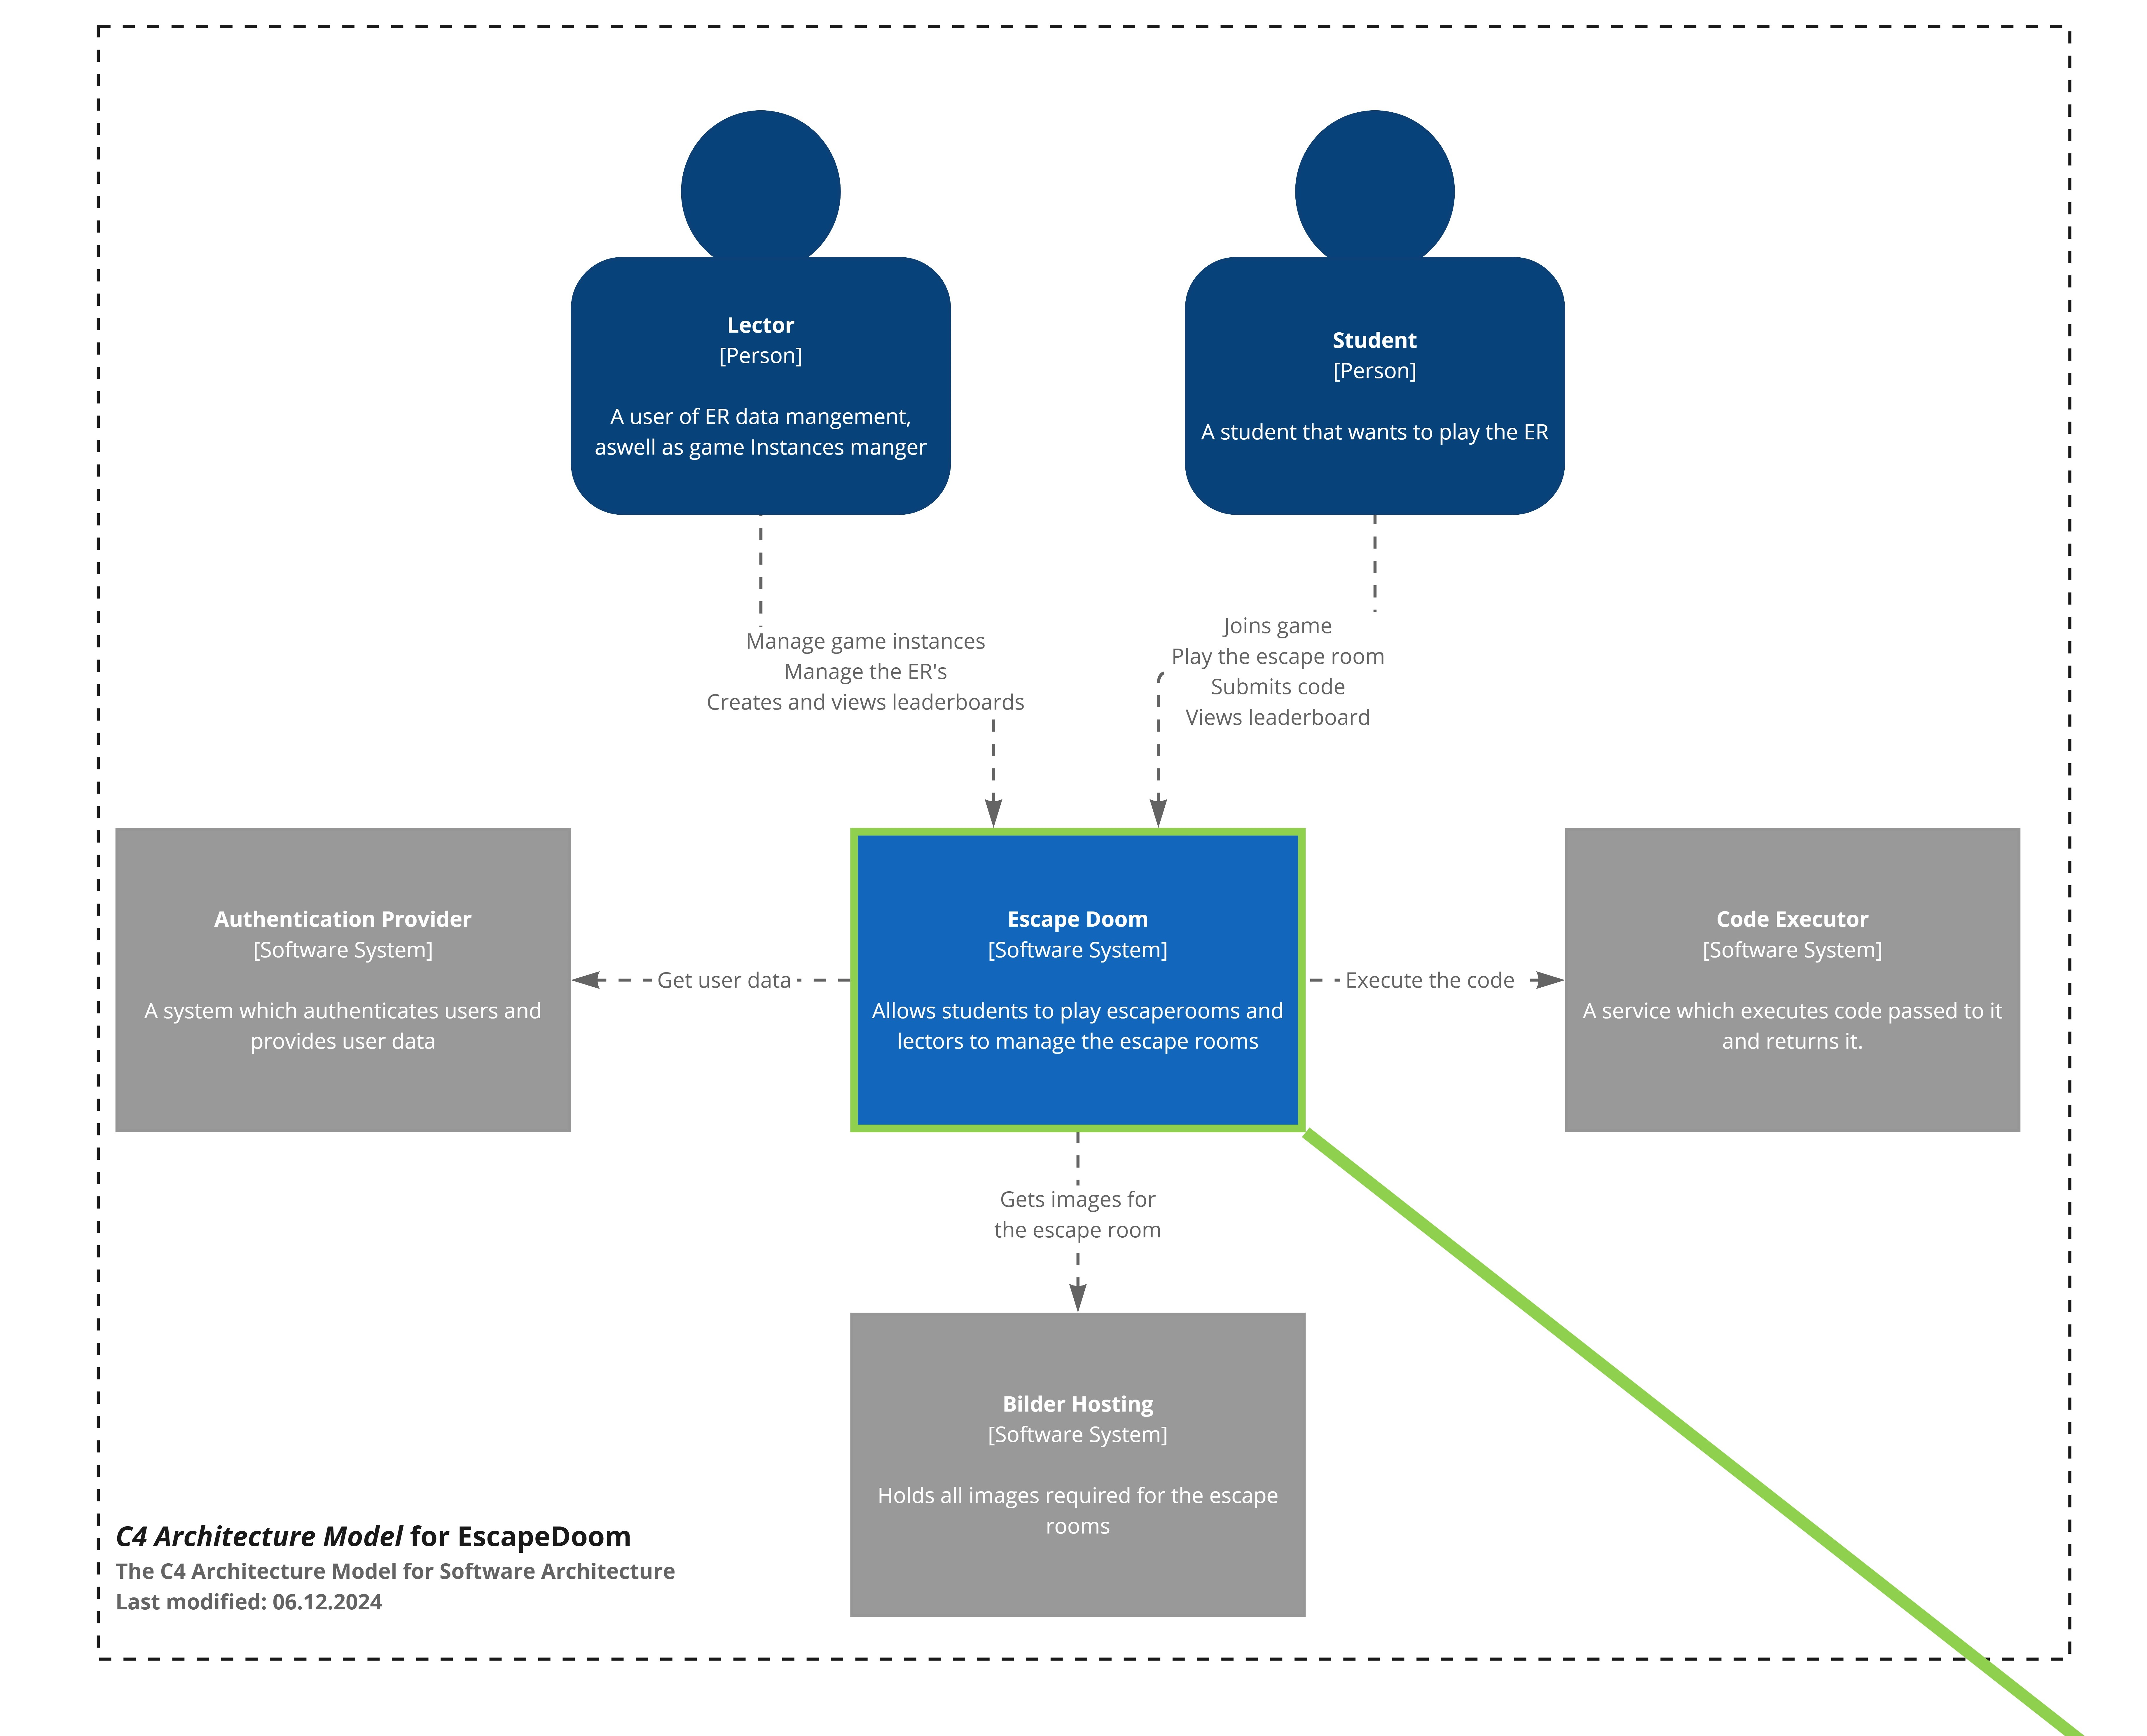
\includegraphics[width=1\linewidth]{images/C4/C1 - EscapeDoom.jpg}
    \caption{Level 1 - Escape Doom}
    \label{fig:c4:c1}
\end{figure}

\begin{table}[h!tbp]
    \centering
    \begin{tabularx}{1\textwidth} {
        | >{\raggedright\arraybackslash}X
        | >{\raggedleft\arraybackslash}X | }
        \hline
        Authentication Provider & Authenticates users to manage access \\
        \hline
        Escpae Doom & The main system, with which the lectors and students interact with \\
        \hline
        Code Executor & Responsible for executing code submitted by students \\
        \hline
        Bilder Hosting & Host images that are displayed in the escape rooms \\
        \hline
    \end{tabularx}
    \caption{Explanation of the individual blocks displayed in the Level 1 Context}
    \label{tab:c4:c1}
\end{table}

\newpage

\subsection{Level 2 - Containers}\label{sub:5:l2}

The EscapeDoom application itself can be segmented into multiple subsystems as depicted in \nameref{fig:c4:c2}. Each dotted line indicates communication, and thus a technical dependency. As can be seen, the front-end is maintained as one application while the back-end is split into micro-services. The are then grouped into three separate domains as can be seen by the dotted lines.

\begin{figure}[h!tbp]
    \centering
    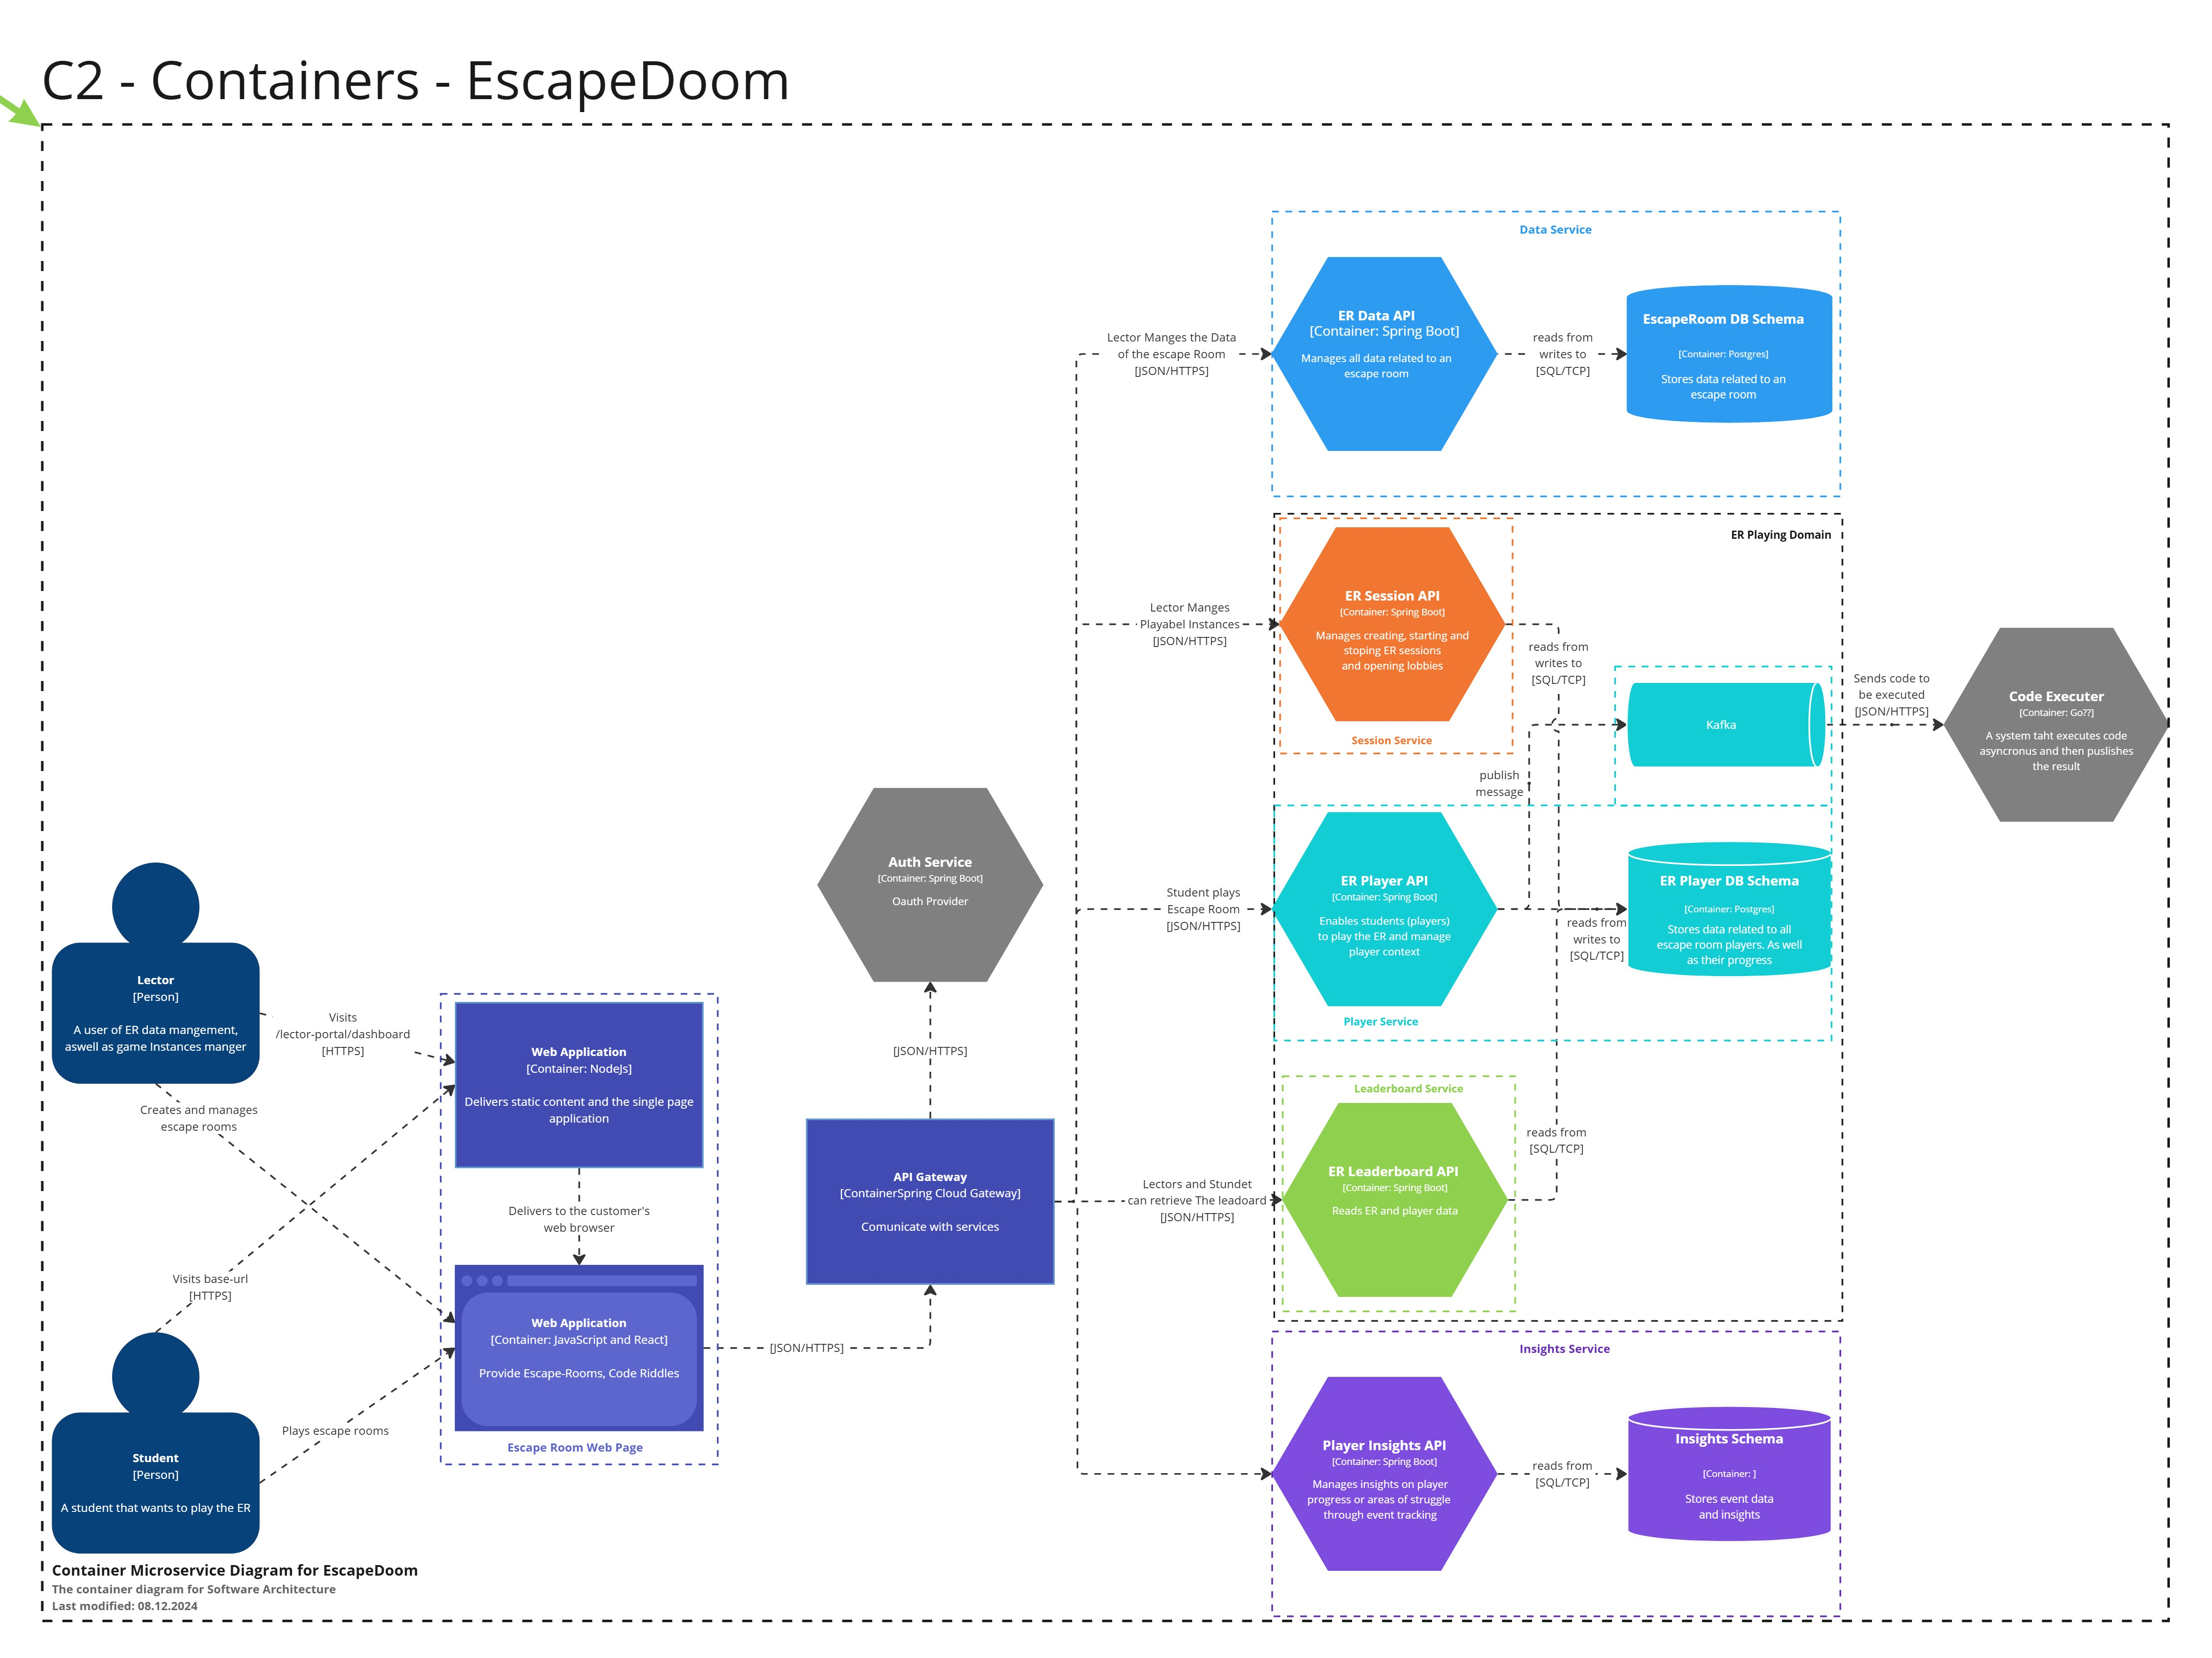
\includegraphics[width=0.9\linewidth]{images/C4/C2 - Containers.jpg}
    \caption{Level 2 - Containers}
    \label{fig:c4:c2}
\end{figure}



\section{Project Tech-Stack}
This project was split into a frontend, based on \href{https://react.dev/}{React} and \href{https://nextjs.org/}{NextJS} and a backend based on \href{https://www.java.com/en/}{Java} and \href{https://spring.io/projects/spring-boot}{SpringBoot}. Below are two images listing most relevant technologies / tools per Stack:

\subsection{Frontend}
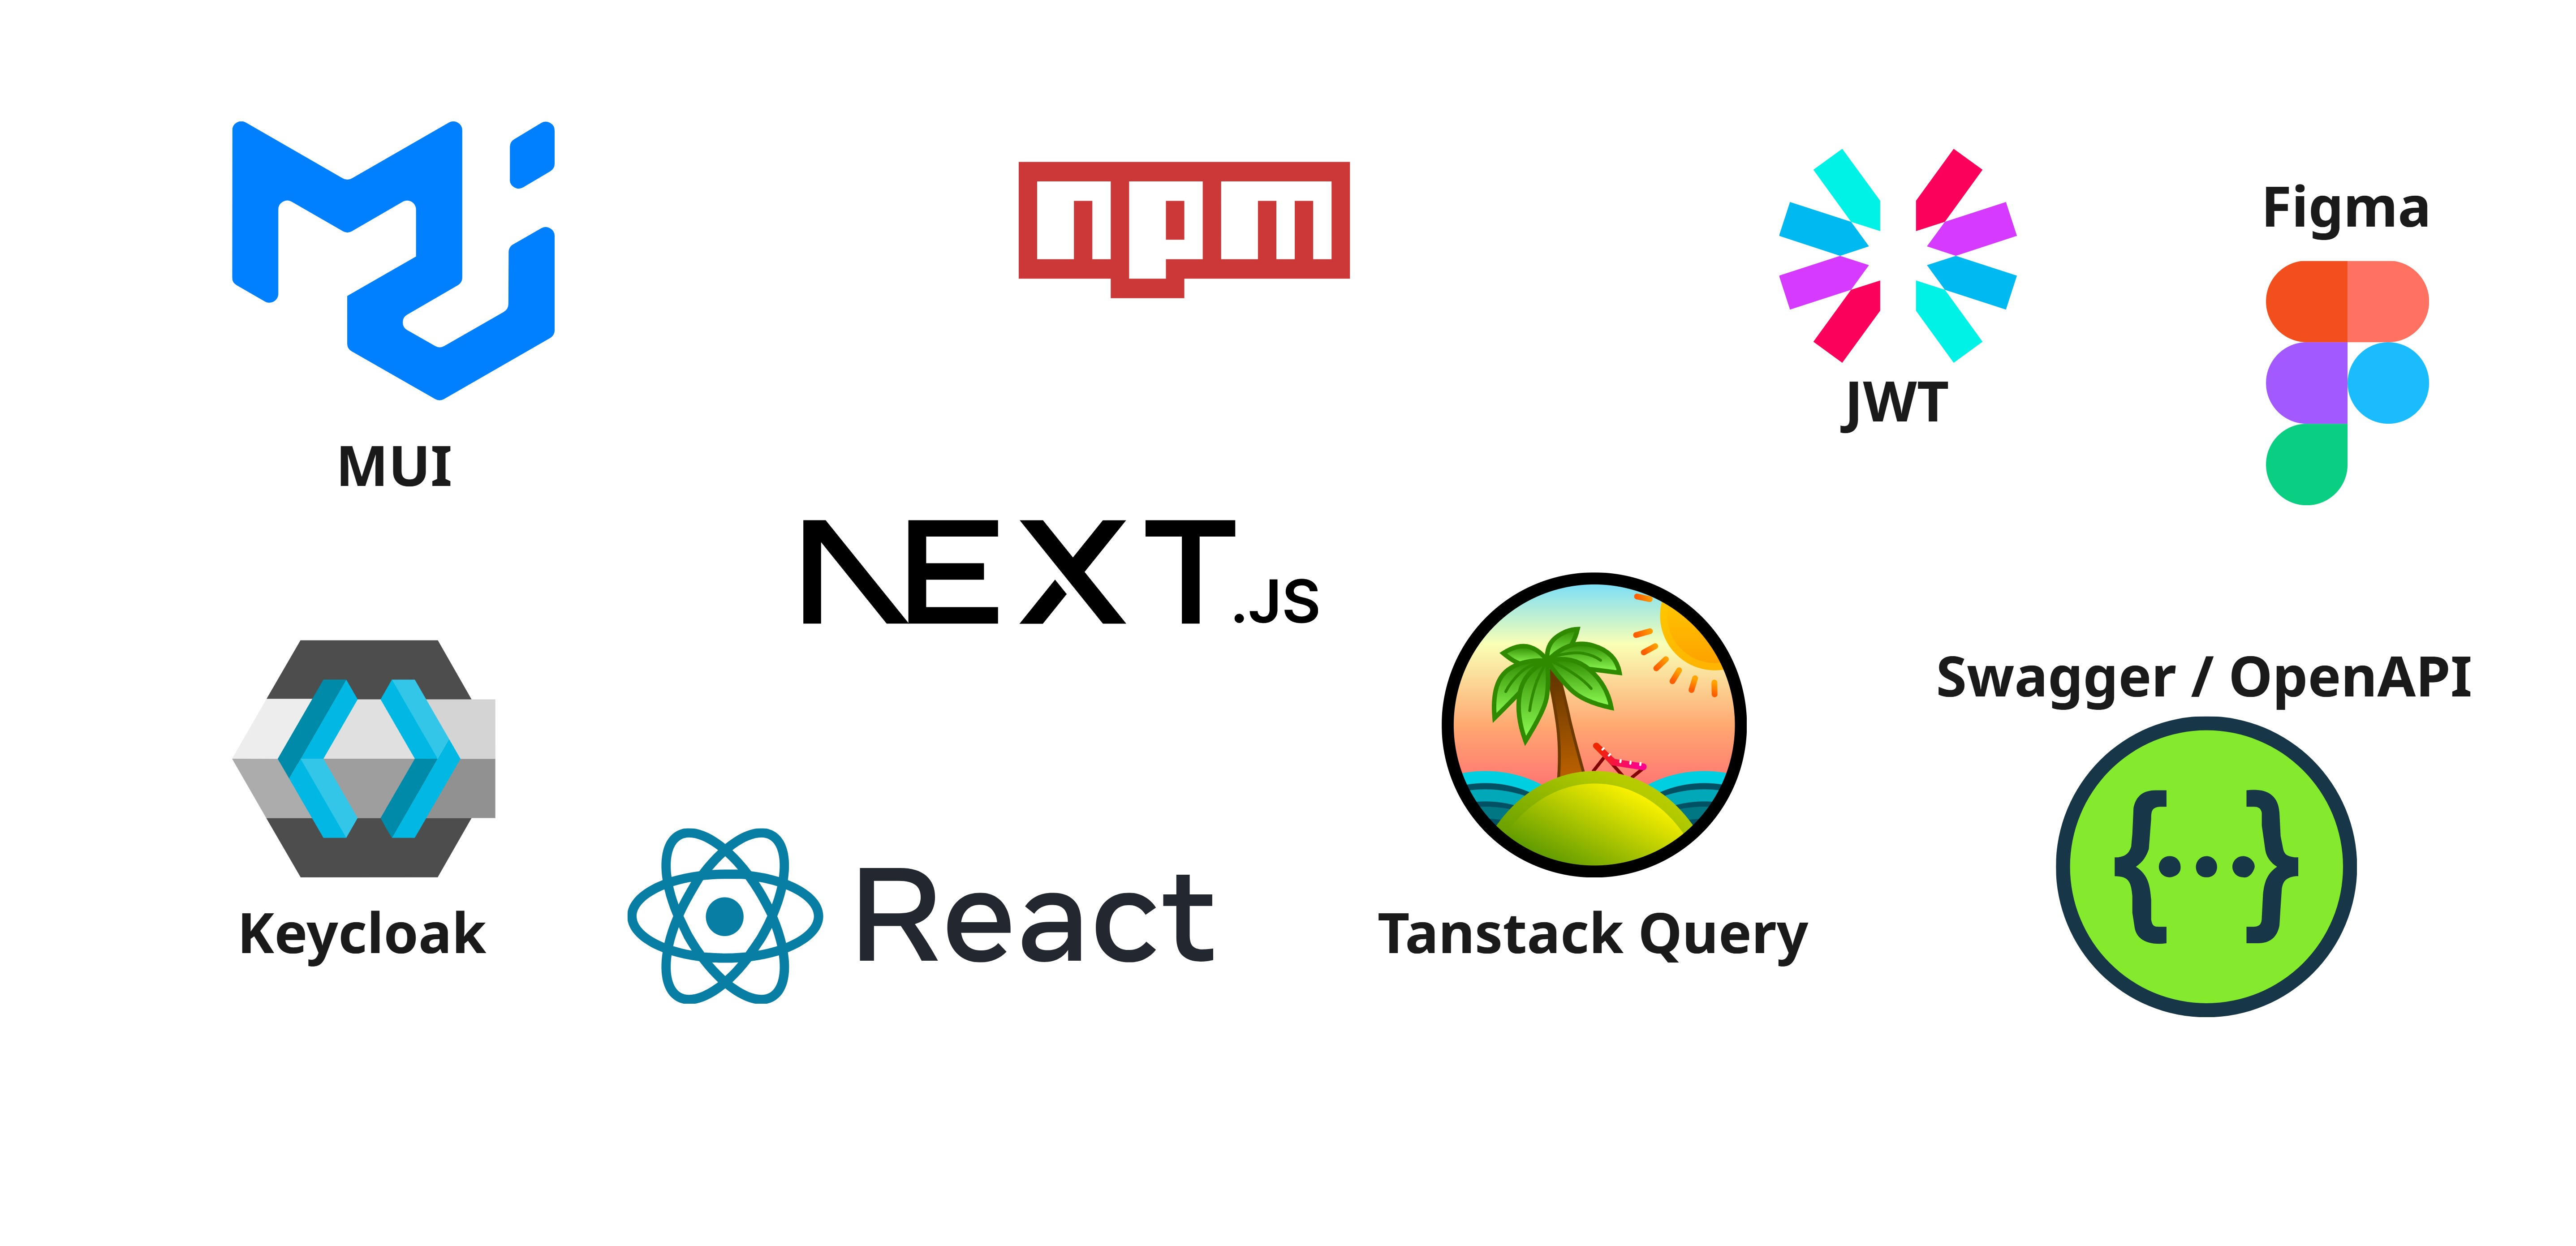
\includegraphics[]{images/SEP1 - EscapeDOOM - Frontend.jpg}

\subsection{Backend}
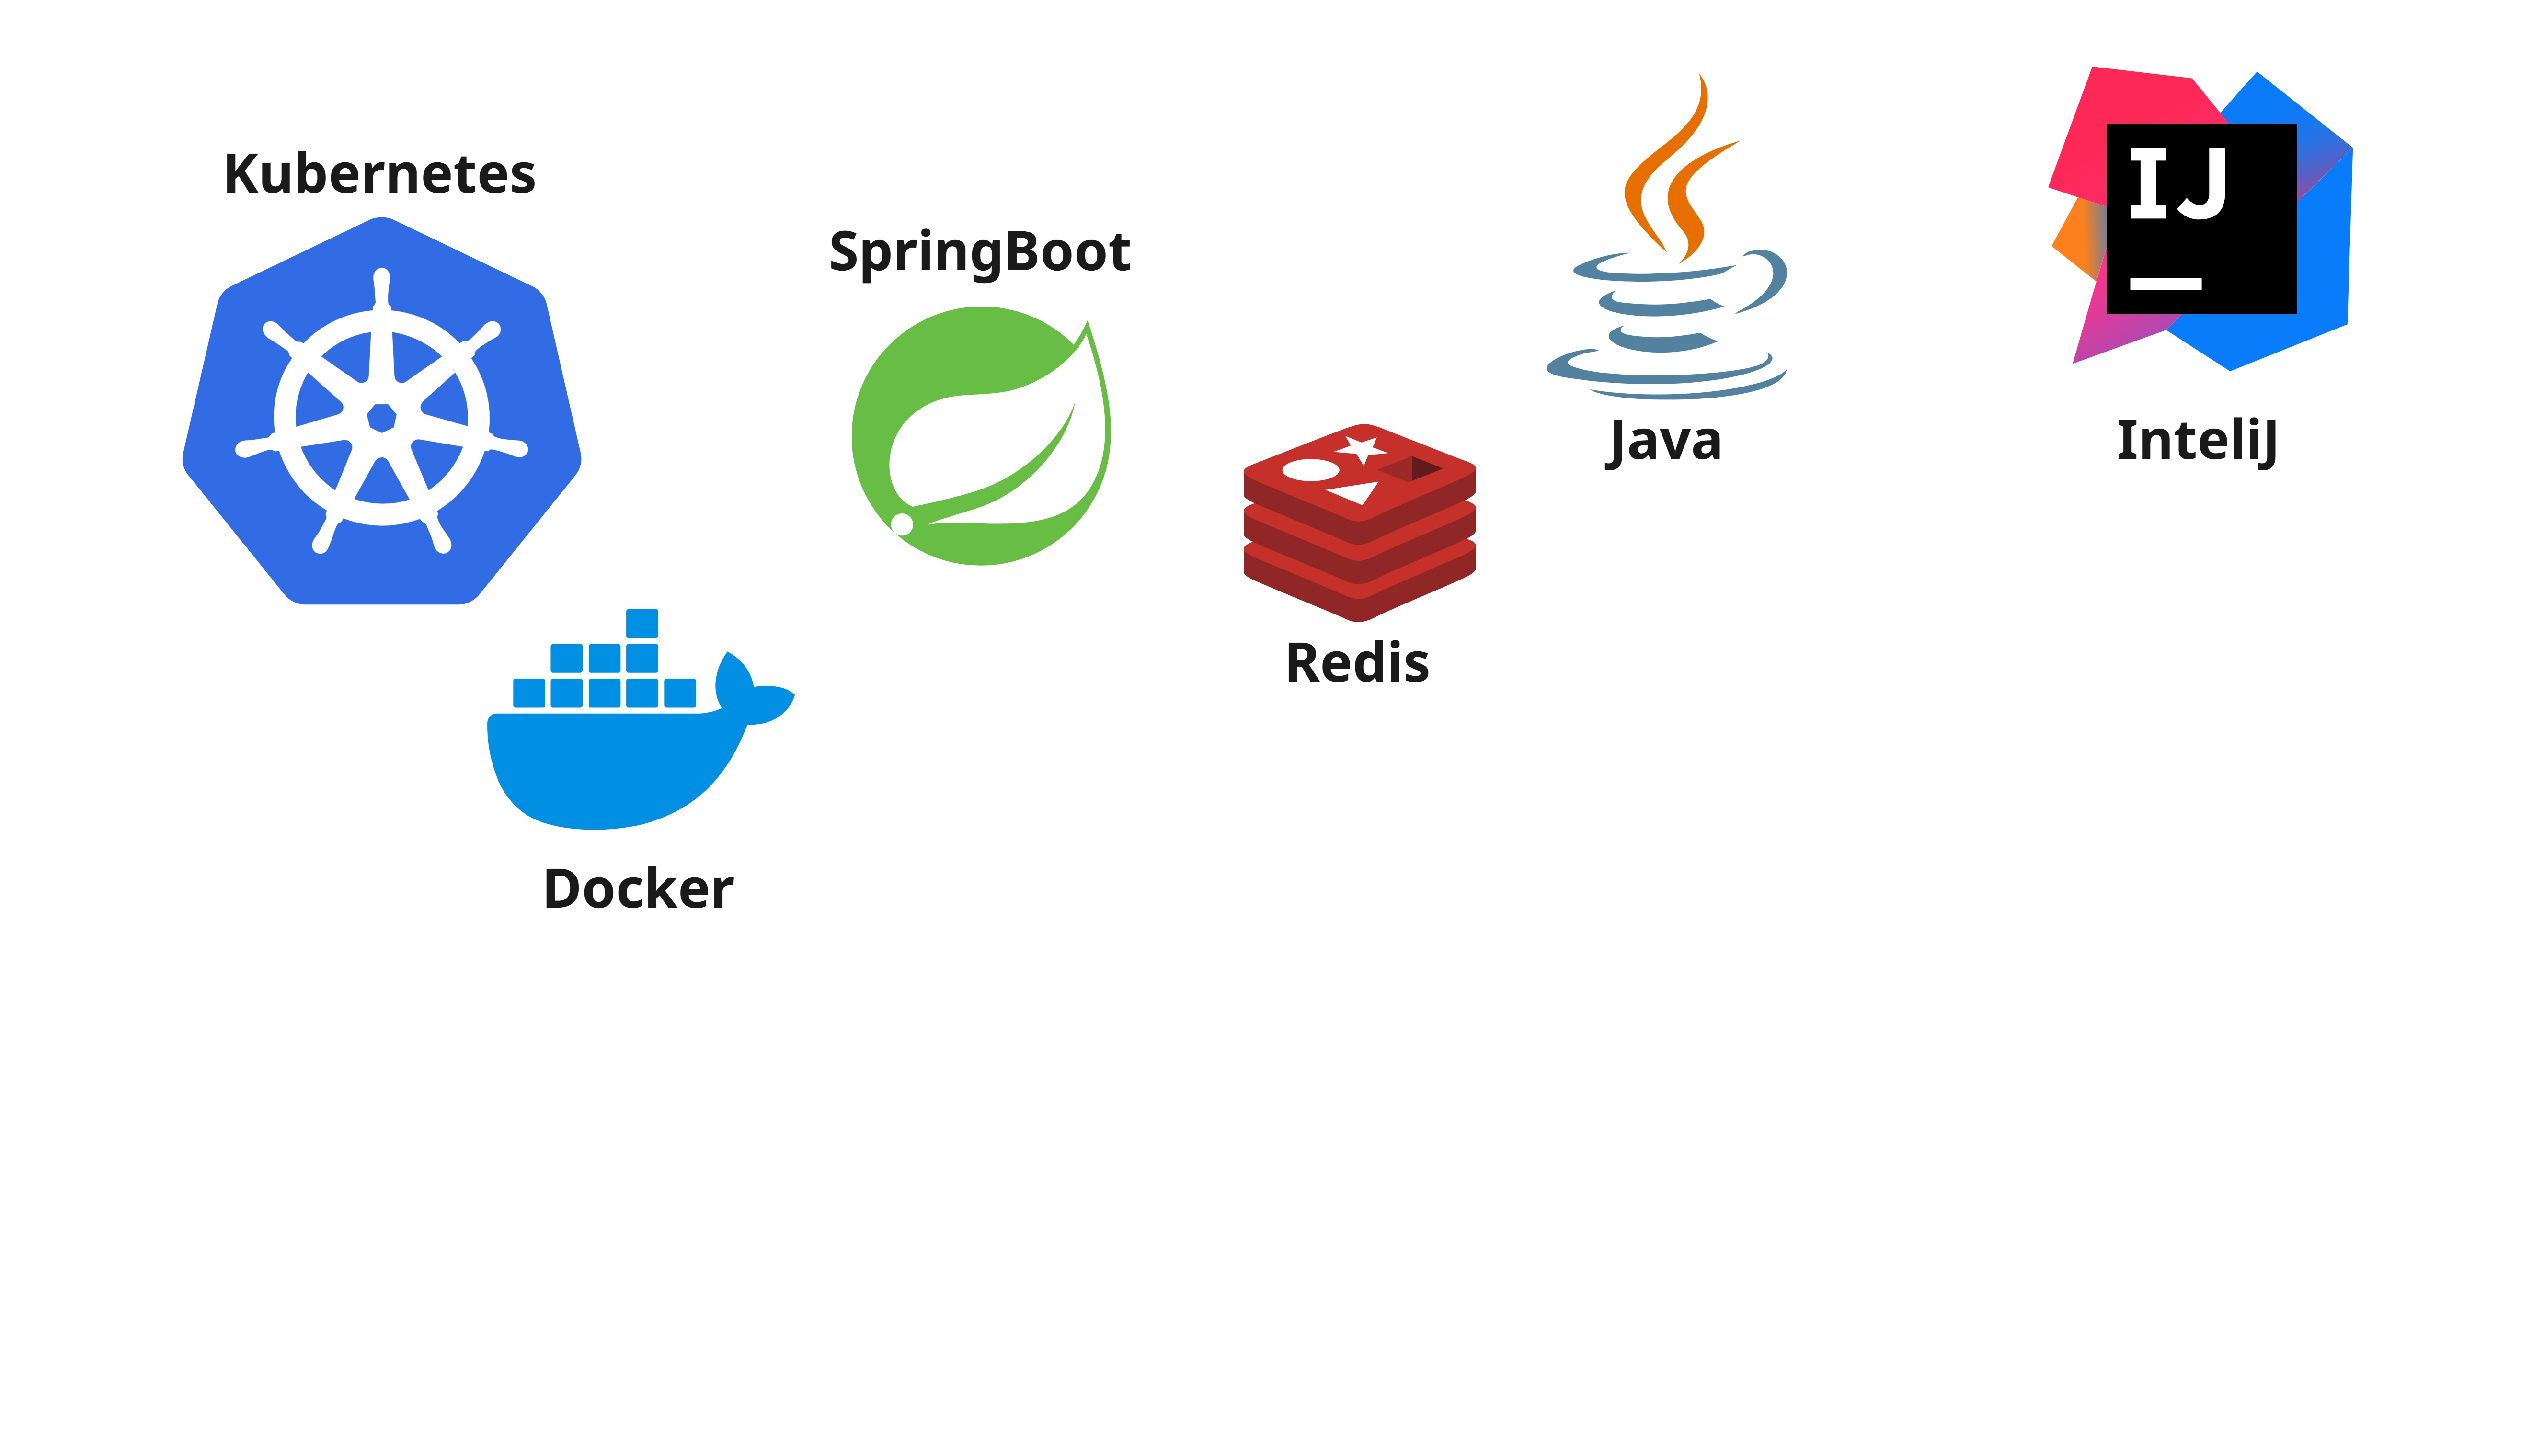
\includegraphics[]{images/SEP1 - EscapeDOOM - Backend.jpg}

\newpage
\subsection{Milestones and current state}
Since this project is a continuation of a bachelor project the first semester of the master, the goals this year was to split the application into microservices, add features and make it a deployable app.

The milestones thus can be split into 5 steps:
\begin{figure}
    \centering
    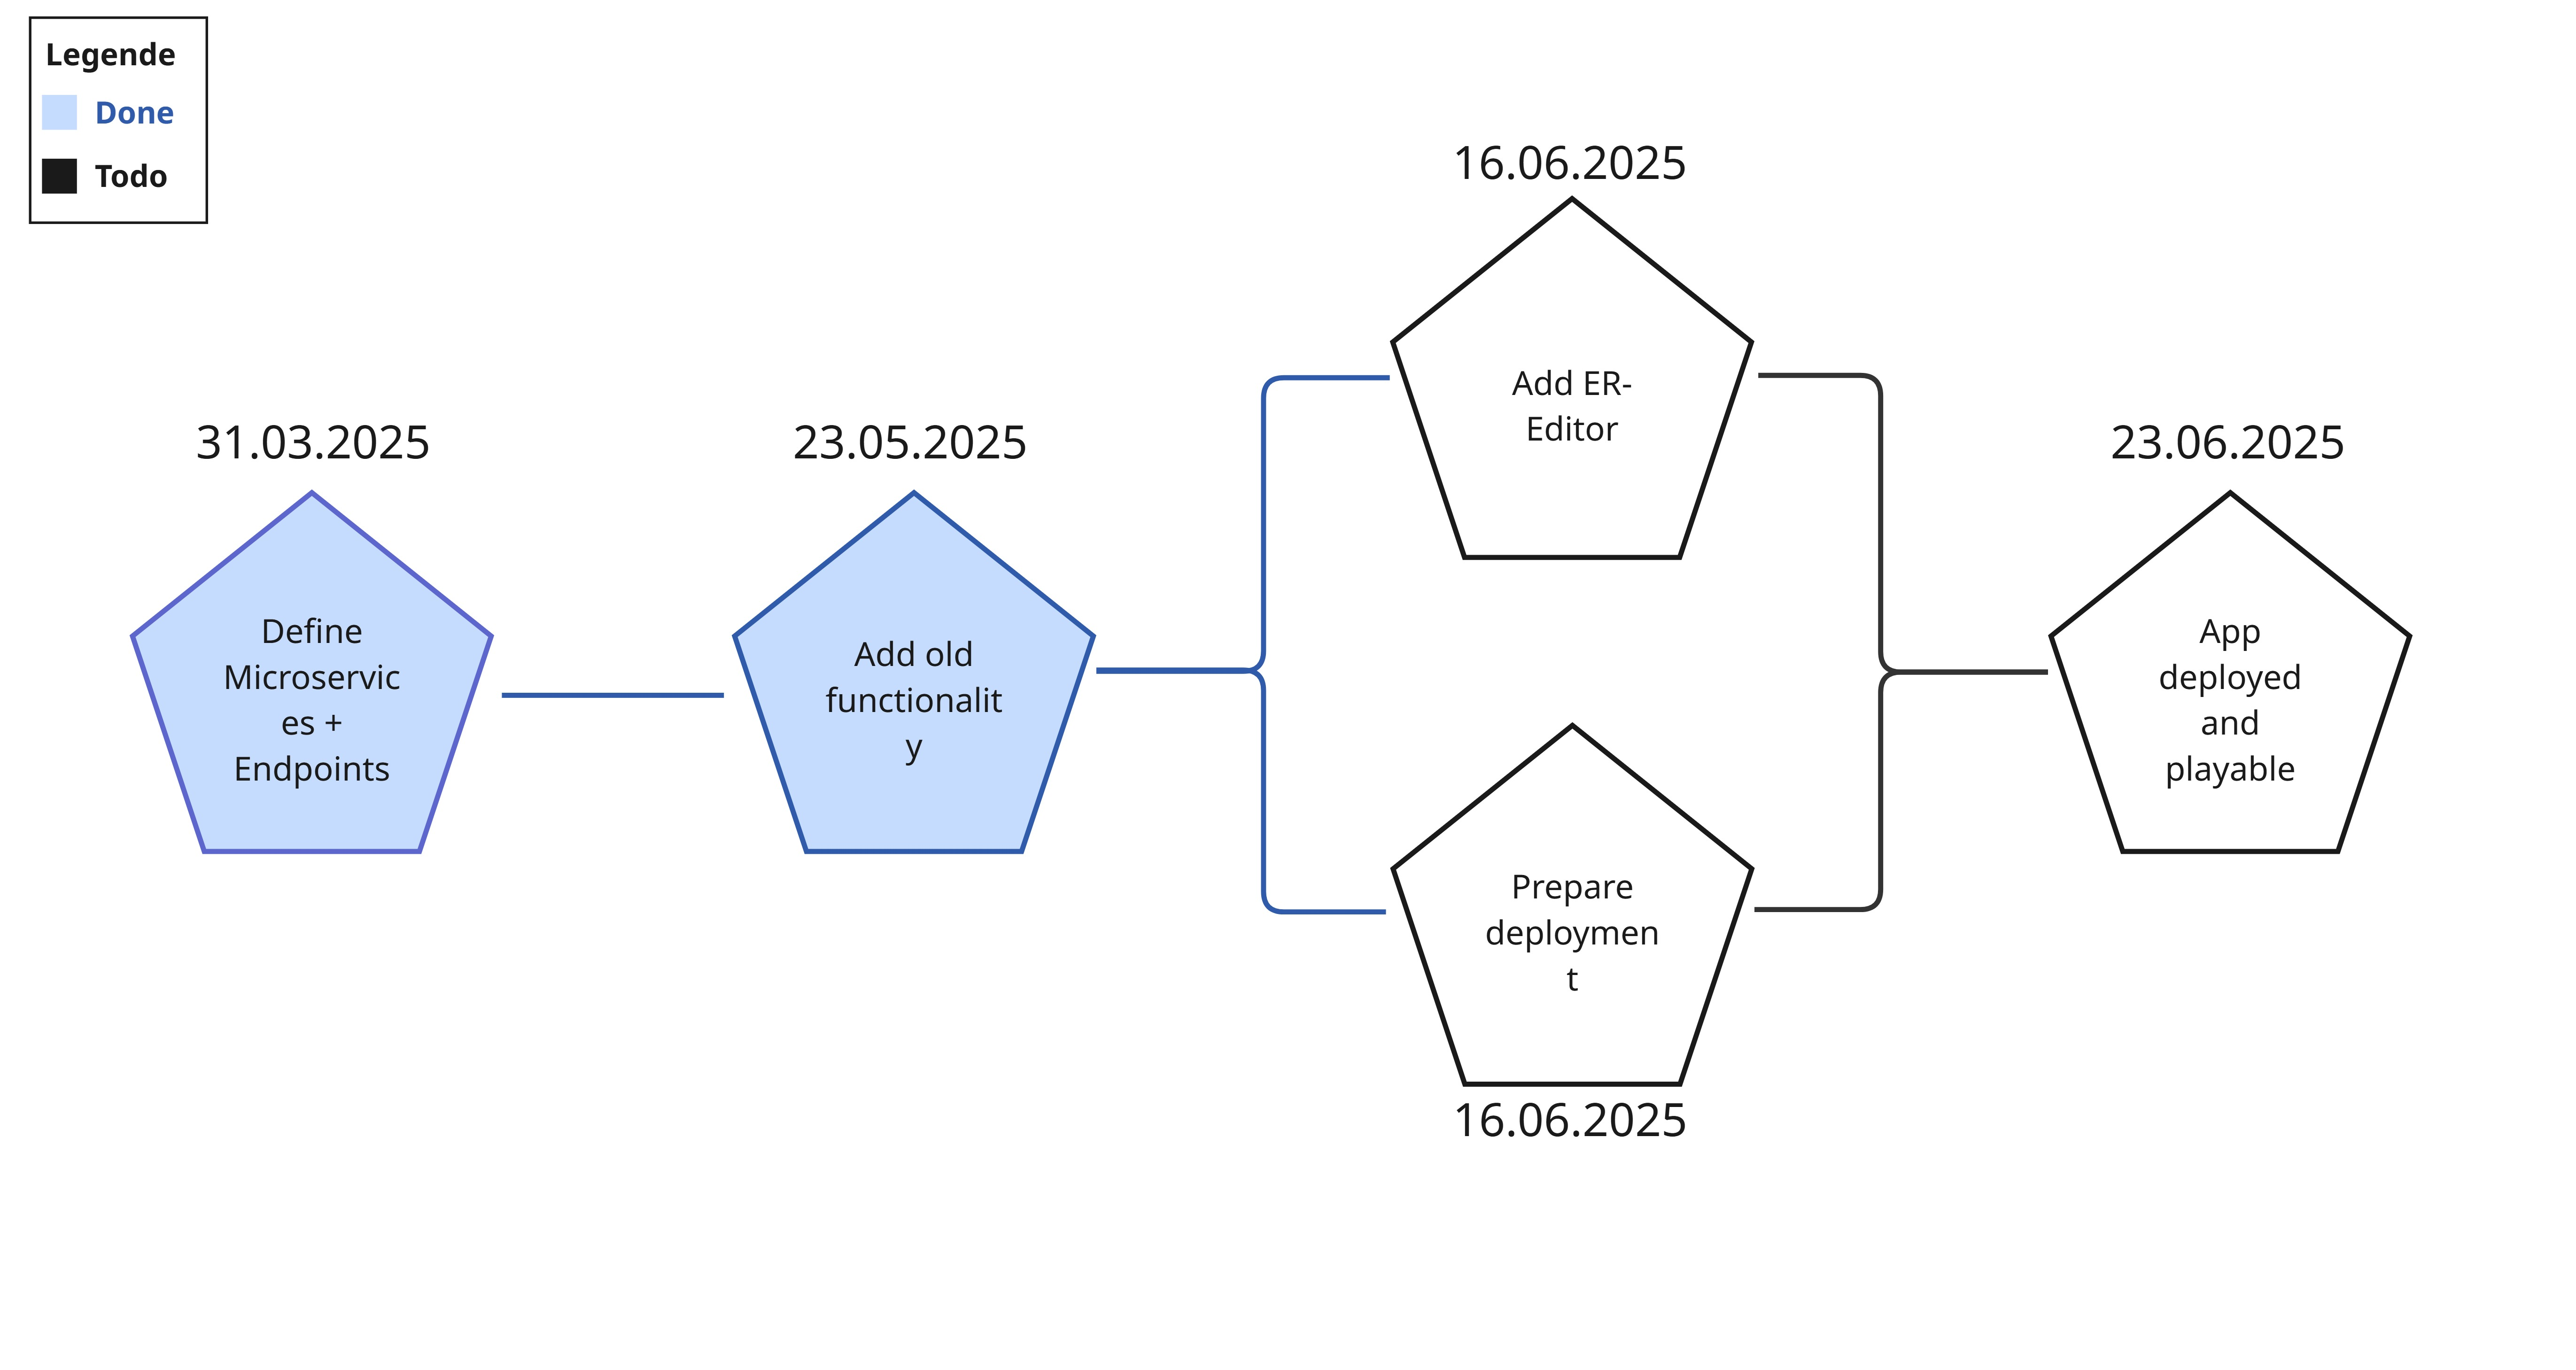
\includegraphics[width=1\linewidth]{images/SEP1 - EscapeDOOM - Milestones.jpg}
\end{figure}

\end{document}
